\documentclass{polytech/polytech}
\usepackage{array}
% zone du préambule

\typereport{custom}
\typereportname{Manuel utilisateur}

\reportyear{2018-2019}

\title{Outil de gestion de parcours patient dans un hôpital de jour}

\schooldepartment{di}
\student[di5]{Romain}{Rousseau}{romain.rousseau@etu.univ-tours.fr}


\motcle{}

\resume{}

\keyword{}

\abstract{}

\begin{document}

\chapter*{Introduction}

Ce document s'adresse aux futurs développeurs du projet d'outil de gestion de patients. Il contient un guide d'installation de l'environnement et de mise en place de la base de données, des informations sur la structure du projet et l'utilisation du framework \textit{CodeIgniter}, et enfin un rapport sur les tests qui ont été réalisés sur l'application ainsi qu'un état sur l'avancée du projet et les suites à donner. 


\chapter{Installation du projet}


\section{Mise en place de l'environnement de développement}

Le projet est sous forme d'application Web. De nombreuses possibilités existent pour développer ce type d'application dans de bonnes conditions selon les préférences du développeur. Pour notre part, nous avons utilisé l'éditeur \textit{Netbeans} qui est particulièrement adapté pour le langage PHP. Nous avons utilisé la version 8.2 pour les développements, mais il existe des versions plus récentes sous la gouverne d'\textit{Apache} depuis fin 2018 (les liens de téléchargements se trouvent ici : \url{https://netbeans.apache.org/download/index.html}).

En ce qui concerne les autres éléments comme la base de données ou le langage PHP, nous avons utilisé WAMP qui est une plate-forme regroupant tous les éléments pour développer des applications web facilement (WAMP est téléchargeable sur le lien suivant : \url{http://www.wampserver.com/}). Le WAMP utilisé pour les derniers développements comportait les versions suivantes :

\begin{itemize}
	\item PHP 5.5.12
	\item Apache 2.4.9
	\item MySQL 5.6.17
\end{itemize}

Par conséquent, il n'est pas recommandé d'utiliser des versions antérieurs à celles décrites précédemment.

\section{Pré-requis}

Pour prendre en main l'application de la meilleure des manières, il est nécessaire d'avoir des bases en développement web (HTML et PHP ici) et surtout de consulter la documentation du framework \textit{CodeIgniter} utilisé pour ce projet. En effet, le framework utilise des concepts et des notions qui lui sont propres (concernant la mise en place des environnements de développement, le chargement des classes, etc.). Le lien de la documentation se trouve sur le lien suivant : \url{https://www.codeigniter.com/user_guide/general/welcome.html}.


\section{Déploiement}

Les sources de l'application sont disponibles sur GitHub à l'adresse suivante :
\url{https://github.com/RomainR37/ParcoursPatient}. Une fois le projet importé, pour déployer l'application sur son poste, il suffit de réaliser les étapes qui suivent : 

\begin{itemize}
	\item Copier toutes les sources dans le dossier \textit{www} de WAMP
	\item Exécuter le script « subway.sql » présent dans le répertoire \textit{BD} du projet dans \textit{PhpMyAdmin} afin de créer et d'ajouter des données à la base 
	\item Lancer le serveur WAMP et aller à l'adresse \url{http://localhost/subway}.
\end{itemize}

La connexion du projet à la base de données se fait au travers du fichier de configuration \textit{database.php} dans le répertoire \textit{app/config}. Veuillez changer les indications du fichier selon votre propre configuration de base de données.

Une fois le déploiement effectif, la page d'accueil de l'application nécessite un login et un mot de passe pour y pénétrer. Le projet étant encore en développement, nous utilisons un utilisateur "administrateur" pour consulter les affichages sur l'application. Ainsi, l'accession avec un compte administrateur se fait avec le nom d'utilisateur \textit{admin} et le mot de passe \textit{admin}.

\chapter{Structure du projet}

L'application web a été développée en utilisant les technologies suivantes :

\begin{itemize}
	\item PHP
	\item HTML, CSS
	\item JavaScript
\end{itemize}

Comme évoqué précédemment, nous avons utilisé le framework PHP \textit{codeIgniter} qui se base sur un modèle MVC (Modèle - Vue - Contrôleur). L'utilité de ce framework est de pouvoir séparer les données des différentes vues permettant l'affichage de ces données. Concernant le CSS, nous avons également utilisé les librairies \textit{bootstrap} utilisées dans bon nombre de sites les plus populaires, afin d'avoir un rendu agréable sans avoir besoin de connaissances poussées dans le domaine.

L'architecture de l'application se présente sous la forme suivante: 

\begin{figure}
	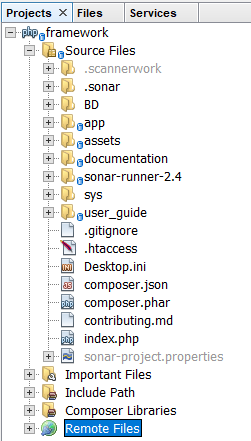
\includegraphics[scale=0.9]{images/arboProjet}
	\caption{Arborescence du projet}
	\label{fig:arboProjet}
\end{figure}

L'arborescence présentée ici est telle qu'elle est retranscrite avec l'IDE \textit{Netbeans}. Les sources de l'application se trouvent au niveau du dossier \textit{app}. Le répertoire \textit{BD} qui contient le script de base de données comme évoqué lors de l'installation précédemment. Ce script contient les tables ainsi que quelques entrées permettant ainsi de commencer dans un environnement déjà prêt à l'emploi.

Le répertoire \textit{assets} contient tous les fichiers images, javascript, css nécessaires à l'affichage de notre application. Le répertoire \textit{documentation} contient la documentation générée avec \textit{ApiGen} afin d'aider à la compréhension du code. Le répertoire \textit{sys} regroupe toutes les classes nécessaires au bon fonctionnement du framework \textit{CodeIgniter}. Et enfin, le répertoire \textit{user\_guide} contient le guide utilisateur du framework \textit{CodeIgniter}.

Par la suite, nous allons nous intéresser à la structure des données dans les fichiers sources, c'est-à-dire dans le répertoire \textit{app}. L'arborescence du programme est présentée comme telle : 

\begin{figure}
	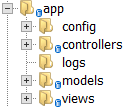
\includegraphics[scale=1]{images/arboMVC}
	\caption{Arborescence du répertoire source}
	\label{fig:arboSource}
\end{figure}

Dans ce répertoire, nous trouvons 5 sous répertoires : 

\begin{itemize}
	\item Config (répertoire de configuration du projet comme la base de données, la mise en place d'environnement, etc.)
	\item Controllers (qui regroupe les contrôleurs de notre application)
	\item Models (avec les données de notre application)
	\item Views (les vues permettant l'affichage des données) 
	\item Tests (avec les tests unitaires du projet)
\end{itemize}

Par la suite, nous allons nous intéresser davantage aux trois parties composant le pattern MVC: les modèles, les vues et les contrôleurs.

\section{Contrôleurs}

Tous les contrôleurs héritent d'une classe CI \textit{Controller} (contrôleur de base du Framework \textit{codeIgniter}). Les contrôleurs permettant de faire le lien entre les données et les vues. Les contrôleurs permettent dans la majeure partie des cas de faire appel à un modèle qui lui-même exécute une requête à la base de données afin d'envoyer les données récupérées à la vue qui se charge de les afficher. 
Nous allons prendre un exemple pour voir l'utilisation d'un contrôleur. 

\begin{figure}
	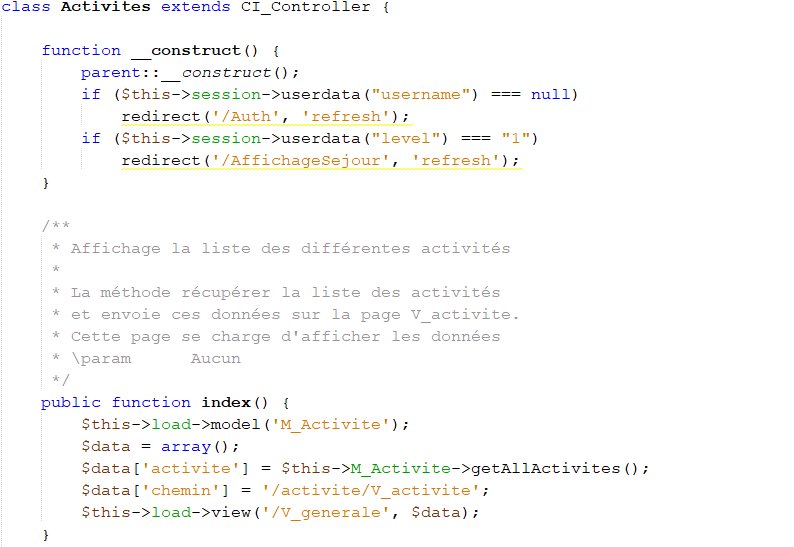
\includegraphics[scale=0.8]{images/controleur}
	\caption{Aperçu d'un contrôleur}
	\label{fig:controleur}
\end{figure}

Dans l'exemple de la \autoref{fig:controleur}, nous prenons le cas du contrôleur \textbf{Activites} et la méthode \textit{index} permettant d'afficher toutes les activités sur une page. La méthode charge le modèle nécessaire à la récupération des différentes activités, nous faisons appel à la méthode \textit{getAllActivites} du modèle \textbf{M\_Activite} permettant de récupérer la liste des activités présentes dans la base de données. Ensuite, nous créons un tableau permettant de récupérer le résultat de la méthode \textit{getAllActivites} avec toutes les activités ainsi que le chemin de la vue des activités qui va nous intéresser par la suite.

Ensuite, notre contrôleur charge la vue principale (voir dans la partie explication des vues pour les détails sur cette partie) en lui donnant également le chemin de la vue \textbf{V\_activite} ainsi que les données provenant du modèle. Tous les contrôleurs et leurs modèles associés sont basés sur une structure de la sorte.

\section{Modèles}

Les modèles exécutent principalement des requêtes vers la base de données. Un exemple avec la \autoref{fig:modele}.

\begin{figure}
	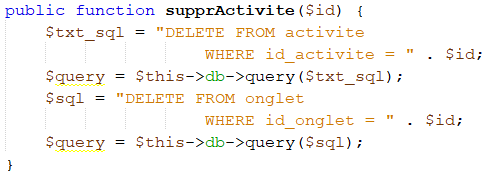
\includegraphics[scale=1]{images/modele}
	\caption{Aperçu d'une fonction d'un modèle}
	\label{fig:modele}
\end{figure}

D'autres fonctions peuvent également être implémentées dans les modèles, de manière générale il s'agit de méthode de vérification des données ou de mise en place propres aux entités qui les concernent. Par exemple, le modèle \textbf{M\_Planning} va contenir des fonctions de mise en place de la planification automatique.


\section{Vues}

Les vues de notre application sont dans le dossier \textit{views}. Chaque vue de notre application dépend d'une vue principale qu'on appelle vue générale (\textbf{V\_generale} dans notre projet). C'est à partir de la vue générale que l'on ajoute le menu, le pied de page ainsi que tous les fichiers js et css nécessaires au fonctionnement de notre application. 

Le schéma de la structure d'une vue se trouve à la \autoref{fig:schemaVues}.

\begin{figure}
	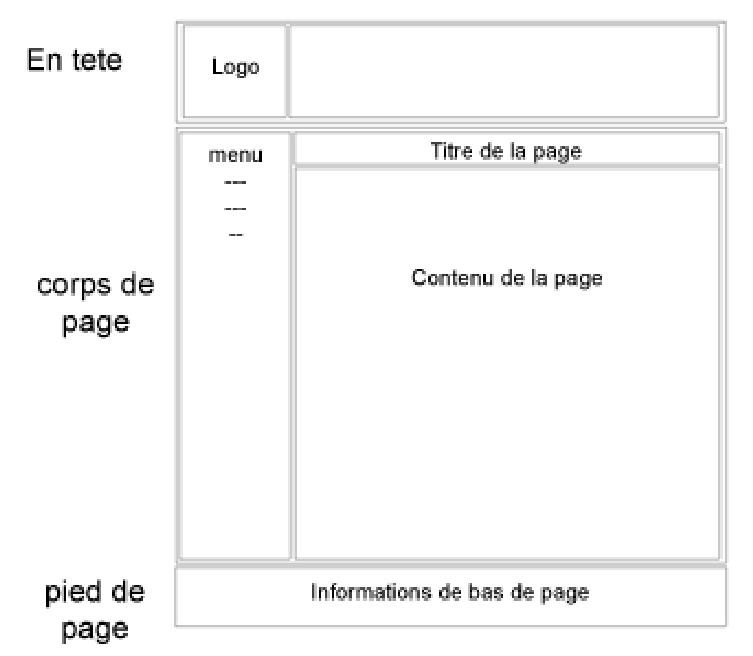
\includegraphics[scale=0.7]{images/schemaVue}
	\caption{Schéma d'une vue}
	\label{fig:schemaVues}
\end{figure}

Dans notre application, chaque vue est reliée à la vue générale, seule la partie contenue de la page est modifiée pour les différents éléments que l'on souhaite aficher. 

Le fonctionnement de ce mécanisme se fait au travers des deux lignes de code présente par la suite.

\begin{figure}
	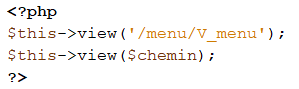
\includegraphics[scale=1]{images/vue}
	\caption{Mécanisme de la vue}
	\label{fig:vue}
\end{figure}

La variable \textit{\$chemin} contient le chemin de la vue permettant d’afficher les données en fonction des actions de l'utilisateur. C'est pour cela que nous devons définir une variable chemin dans nos différentes méthodes de nos contrôleurs. 

\chapter{Rapport de tests}

Ce rapport présente les tests unitaires réalisés sur l'application ainsi que les tests de fiabilité pour attester du fonctionnement de la planification automatique des patients sur le calendrier.

\section{Mise en place des tests}

La partie concernée par les tests mises en place au cours de derniers développements est basée sur la planification automatique des patients par jour car il s'agit de la partie la plus complexe à mettre en place. Pour l'occasion, nous avons mis en place des tests unitaires d'un côté pour vérifier le bon fonctionnement des méthodes, et des tests de fiabilité de l'autre pour voir si la planification est viable pour certains volumes de données.

\subsection{Tests unitaires}

Les tests unitaires ont été réalisés avec \textit{PHPUnit} au travers d'un module adapté à \textit{CodeIgniter} intitulé \textit{ci-phpunit-test}. Ce module a été ajouté dans le projet et il n'est pas nécessaire de le re-télécharger pour les prochains développements. 

Le fonctionnement de \textit{PHPUnit} se trouve dans la documentation en suivant le lien : \url{https://phpunit.readthedocs.io/fr/latest/index.html}. Pour ce qui est du module \textit{ci-phpunit-test}, le projet se trouve sur le répertoire GitHub suivant : \url{https://github.com/kenjis/ci-phpunit-test}, dans lequel une documentation complète est disponible.

\subsection{Tests de fiabilité}

Des tests de fiabilité ont été mis en place afin de voir si la planification telle qu'implémentée ici est viable ou non. Pour tester la planification, nous nous sommes basés sur les données fournies par l'AP-HP qui nous permettent d'avoir des informations sur les ressources matérielles à disposition et sur le nombre de patients qui peuvent être pris en charge sur une journée. Aussi, pour ses tests, nous nous sommes focalisés sur un secteur précis de l'hôpital, à savoir les traitements de l'obésité, afin d'avoir un aperçu sur les partages de ressources communes à plusieurs patients. 

Les parcours sont distingués par des codes : P1, P2 et P3, et certaines abréviations sur les ressources peuvent apparaître. Ceux-ci sont détaillés dans le rapport de PR\&D complet.

Par conséquent, voici les données d'entrée des tests:

\begin{itemize}
	\item 9 patients disponibles de 8h à 20h: 4 sur le parcours P1, 2 sur le parcours P2 et 3 sur le parcours P3
	\item Le personnel est composé de : 3 IDE obésité, 4 IDE, 2 psychologues, 3 diététiciens, 3 nutritionnistes, 2 internes obésité et 1 médecin hépato.
	\item L'hôpital dispose des salles suivantes : 2 box prélèvement, 4 HDJ obésité et 5 bureaux CS.
\end{itemize}

À partir de ces données, nous avons pu obtenir les résultats de la partie qui suit.

\section{Résultats des tests}

\subsection{Tests unitaires}

5 tests unitaires ont été réalisés : 

\begin{description}
	\item[test\_getCouleurEventPatient()] : teste la méthode qui récupère la couleur des événements d'un patient. Ce test est présent en particulier pour vérifier si les appels à la base fonctionnent correctement.
	\item[test\_addEvenementAuto()] : teste la méthode d'ajout d'événement automatique c'est-à-dire sans préciser de ressource. Pour ce test, l'évènement que l'on souhaite ajouter est lié à deux ressources, ainsi 2 entrées doivent être créées dans la table "evenement". La table "evenement" doit être vide avant le test.
	\item[test\_getDisponibiliteRessource()] : teste la méthode de disponibilité d'une ressource. Un évènement est ajouté pour la ressource 1 entre 8h30 et 8h50. Teste la méthode \textit{getDisponibiliteRessource()} avec plusieurs horaires en paramètre afin de vérifier si la méthode renvoie les bons résultats.
	\item[test\_planautoCreationEvenement()] : vérifie que l'appel à la méthode de planification crée bien des événements.
	\item[test\_planautoAjoutPatient] : teste la planification automatique pour un patient suivant le parcours 1 (Obésité sévère diagnostic). 11 activités doivent être réalisées sur ce parcours, chacune avec deux ressources excepté deux activités avec 1 ressource seulement. Au total, 20 évènements (9*2 + 2) doivent être présents dans la base après application de la méthode.
\end{description}

Le détail des tests se trouvent sur le répertoire \textit{/app/tests} du projet.

Comme on le voit sur l'image suivante, tous les tests ont été passés avec succès.

\begin{figure}
	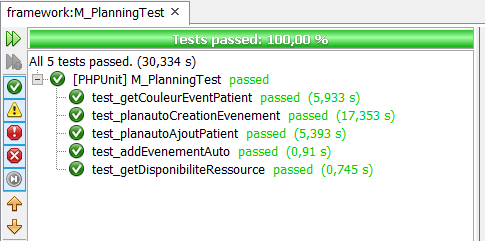
\includegraphics[scale=0.85]{images/testsPassed}
	\caption{Tests unitaires}
	\label{fig:testsunit}
\end{figure}

\subsection{Tests de fiabilité}

\begin{longtabu}{|X||X||X||X[0.4,c]|}
	\hline
	\textbf{Tests de planification} & \textbf{Résultats attendus} & \textbf{Résultats obtenus} & \textbf{Etat du test} \\
	\hline
	\endhead
	\hline
	1 patient sur le parcours P1 & Aucune erreur de précédence & Aucune erreur de précédence & OK \\
	\hline
	1 patient sur le parcours P1 & Respect des disponibilités du patient & Respect des disponibilités du patient & OK \\
	\hline
	1 patient sur le parcours P1 & Aucune activité n'a lieu au même moment & Aucune activité n'a lieu au même moment & OK \\
	\hline
	1 patient sur le parcours P1 & Le parcours commence dès la première disponibilité du patient & Le parcours commence dès la première disponibilité du patient & OK \\
	\hline
	1 patient sur le parcours P1 & Toutes les activités sont planifiées & Toutes les activités sont planifiées & OK \\
	\hline
	\hline
	2 patients sur la parcours P1 & Aucune erreur de précédence & Aucune erreur de précédence & OK \\
	\hline
	2 patients sur le parcours P1 & Respect des disponibilités des patients & Respect des disponibilités des patients & OK \\
	\hline
	2 patients sur le parcours P1 & Aucune ressource n'est attribuée sur 2 activités en simultanée & Aucune ressource n'est attribuée sur 2 activités en simultanée & OK \\
	\hline
	2 patients sur le parcours P1 & Toutes les activités sont planifiées & Toutes les activités sont planifiées & OK \\
	\hline
	\hline
	... Les tests entre 3 et 6 patients sont concluants & & & OK \\
	\hline
	\hline
	7 patients à planifier & Aucune erreur de précédence & Aucune erreur de précédence & OK \\
	\hline
	7 patients à planifier & Respect des disponibilités des patients & Le patient 7 a des activités hors de ses disponibilités & \textbf{Échec} \\
	\hline
	7 patients à planifier & Aucune ressource n'est attribuée sur 2 activités en simultanée & Aucune ressource n'est attribuée sur 2 activités en simultanée & OK \\
	\hline
	7 patients à planifier & Toutes les activités sont planifiées & Toutes les activités sont planifiées & OK \\
	\hline
	\hline		
\end{longtabu}

Suite aux tests, plusieurs constats peuvent être effectués. Parmi les éléments qui fonctionnent correctement quelque soit le nombre de patients, nous avons : 

\begin{itemize}
	\item Toutes les activités sont placées sur la calendrier
	\item Les précédences entre activité sont respectées
	\item Aucune ressource n'est utilisée par plusieurs activités simultanément
\end{itemize}

Ensuite parmi les éléments à revoir, dès que l'on dépasse la limite de 6 patients dans notre cas de test, les suivants débordent sur la fin du calendrier. Cela ne laisserait que très peu de marges de manœuvre pour l'hôpital puisque, d'après leurs données fournies, ils prévoient d'accueillir 6 patients par jour sur les parcours utilisés pour les tests ici. Un autre aspect à prendre en compte et qui ne figure pas dans les tests précédents est le temps d'attente des patients qui décuple au fil de la journée.

La planification telle qu'implémentée ici utilise les premières ressources disponibles pour l'attribution des activités, ce qui entraîne des taux d'occupation entre ressources totalement disparates. La première ressource sera utilisée systématiquement dès qu'elle est disponible tandis que la dernière peut ne jamais être utilisée dans la journée. 

Une correction importante à apporter est la planification automatique alors qu'une activité a été placée manuellement sur le calendrier. Dans ce cas, la planification résultante sera toujours fausse, ce qui est à corriger.

Malgré les problèmes constatés sur cette méthode, il est important de noter qu'il s'agit seulement de la première mouture de la planification. Celle-ci a été pensée telle que l'on prenne en compte les activités patient par patient et sans aucune optimisation supplémentaire. Le but premier qui est de proposer une solution directe de planification à la personne en charge est atteint.

\end{document}